
%(BEGIN_QUESTION)
% Copyright 2007, Tony R. Kuphaldt, released under the Creative Commons Attribution License (v 1.0)
% This means you may do almost anything with this work of mine, so long as you give me proper credit

{\it Integral} control action is where the output signal of a controller changes at a rate directly proportional to the magnitude of {\it error} (the difference between process variable and setpoint).

Given this definition, identify how a integral-acting controller would respond to the following process variable (PV) and setpoint (SP) values over time:

$$\includegraphics[width=15.5cm]{i02418x01.eps}$$

Assume {\it direct} control action.

\underbar{file i02418}
%(END_QUESTION)





%(BEGIN_ANSWER)

With integral action, the amount of error tells the output how {\bf fast} to go:

$$\includegraphics[width=15.5cm]{i02418x02.eps}$$

%(END_ANSWER)





%(BEGIN_NOTES)


%INDEX% Control, integral: defined

%(END_NOTES)


